% Figure 13.3: a representative collection of virtual soft-photon corrections.
% Source: physical PDF p. 563 (printed p. 540).
\usetikzlibrary{decorations.pathreplacing}
\begingroup
\renewcommand{\thefigure}{13.\arabic{figure}}
\setcounter{figure}{2}
\begin{figure}[tbp]
\centering
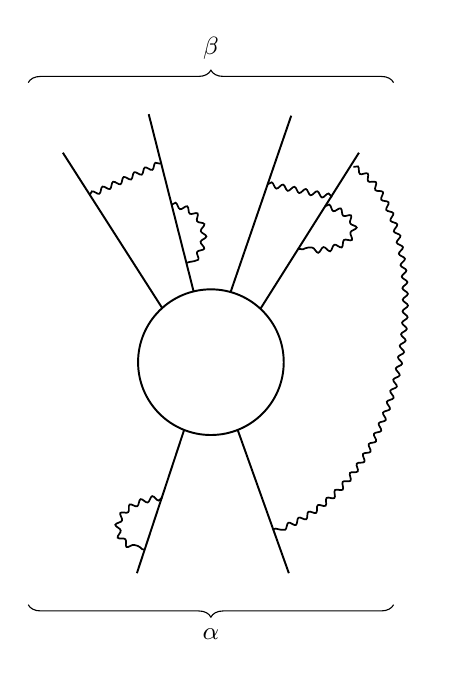
\begin{tikzpicture}[
  particle/.style={line width=0.7pt},
  photon/.style={line width=0.62pt,decorate,
    decoration={snake,amplitude=0.95pt,segment length=4.2pt}},
  hard/.style={draw,line width=0.7pt,circle,minimum size=1.85cm,inner sep=0pt},
  statebrace/.style={decorate,decoration={brace,amplitude=4.5pt}},
  every node/.style={font=\small}
]
  \node[hard] at (0,0) {};
  \draw[particle] (-0.62,0.69) -- (-1.88,2.66);
  \draw[particle] (-0.22,0.90) -- (-0.79,3.15);
  \draw[particle] (0.25,0.89) -- (1.02,3.13);
  \draw[particle] (0.63,0.68) -- (1.88,2.66);
  \draw[particle] (-0.34,-0.86) -- (-0.94,-2.68);
  \draw[particle] (0.34,-0.86) -- (0.99,-2.68);

  % Six virtual soft-photon attachments visible in the source.
  \draw[photon] (-1.54,2.12) -- (-0.63,2.53);
  \draw[photon] (-0.50,2.00) .. controls (0.03,1.91) and (-0.10,1.35) .. (-0.31,1.26);
  \draw[photon] (0.72,2.26) -- (1.54,2.10);
  \draw[photon] (1.45,1.98) .. controls (2.02,1.85) and (1.82,1.35) .. (1.11,1.44);
  \draw[photon] (1.81,2.48) .. controls (2.80,1.93) and (2.73,-1.45) .. (0.80,-2.12);
  \draw[photon] (-0.62,-1.72) .. controls (-1.25,-1.78) and (-1.30,-2.30) .. (-0.84,-2.38);

  \draw[statebrace] (-2.32,3.55) -- (2.32,3.55)
    node[midway,above=5pt] {$\beta$};
  \draw[statebrace,decoration={brace,amplitude=4.5pt,mirror}]
    (-2.32,-3.08) -- (2.32,-3.08)
    node[midway,below=5pt] {$\alpha$};
\end{tikzpicture}
\caption{A typical dominant graph for the radiative corrections due to virtual soft photons to the $S$-matrix for the process $\alpha\to\beta$. Straight lines are particles in the states $\alpha$ and $\beta$ (including possible hard photons); wavy lines are soft photons.}
\label{fig:weinberg-13-3}
\end{figure}
\endgroup
